%% !TEX root = ../../handbook-physics.tex
%%!TEX TS-program = pdflatex
%%!TEX encoding = UTF-8 Unicode

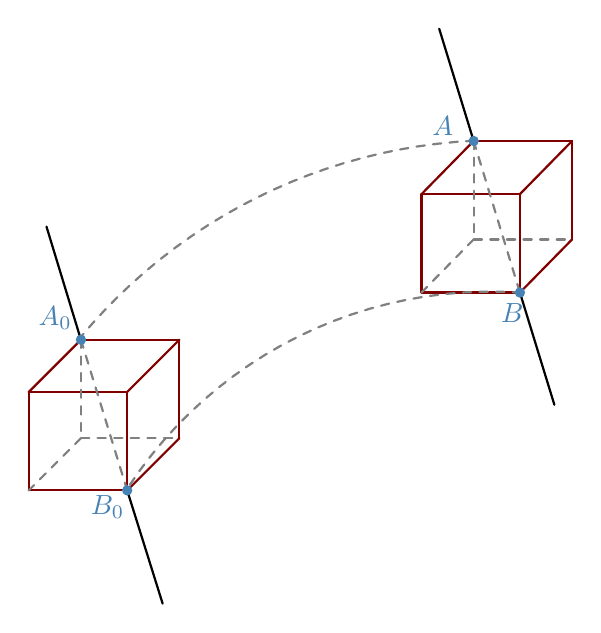
\begin{tikzpicture}[line cap=round,line join=round,scale=1.25]
\draw[thick,Maroon] (0.99,5.01) -- (0.99,4.01);% -- (1.99,4.01) -- (1.99,5.01);
\draw [thick,Maroon] (-3.,3.)-- (-3.,2.);
\draw [thick,color=Maroon] (-3.,2.)-- (-2.,2.);
\draw [thick,color=Maroon] (-2.,2.)-- (-2.,3.);
\draw [thick,color=Maroon] (-2.,3.)-- (-3.,3.);
\draw [thick,dashed,color=gray] (-2.47,3.53)-- (-2.47,2.53);
\draw [thick,dashed,color=gray] (-2.47,2.53)-- (-1.47,2.53);
\draw [thick,color=Maroon] (-1.47,2.53)-- (-1.47,3.53);
\draw [thick,color=Maroon] (-1.47,3.53)-- (-2.47,3.53);
\draw [thick,color=Maroon] (-2.47,3.53)-- (-3.,3.);
\draw [thick,color=Maroon] (-1.47,3.53)-- (-2.,3.);
\draw [thick,color=Maroon] (-1.47,2.53)-- (-2.,2.);
\draw [thick,dashed,color=gray] (-2.47,2.53)-- (-3.,2.);
\draw [thick,color=Maroon] (0.99,4.01)-- (1.99,4.01);
\draw [thick,color=Maroon] (1.99,4.01)-- (1.99,5.01);
\draw [thick,color=Maroon] (1.99,5.01)-- (0.99,5.01);
\draw [thick,dashed,color=gray] (1.52,5.55)-- (1.52,4.55);
\draw [thick,dashed,color=gray] (1.52,4.55)-- (2.52,4.55);
\draw [thick,color=Maroon] (2.52,4.55)-- (2.52,5.55);
\draw [thick,color=Maroon] (2.52,5.55)-- (1.52,5.55);
\draw [thick,color=Maroon] (1.52,5.55)-- (0.99,5.01);
\draw [thick,color=Maroon] (2.52,5.55)-- (1.99,5.01);
\draw [thick,color=Maroon] (2.52,4.55)-- (1.99,4.01);
\draw [thick,dashed,color=gray] (1.52,4.55)-- (0.99,4.01);
\draw [shift={(1.80,0.)},thick,dashed,color=gray]  plot[domain=1.62:2.45,variable=\t]({1.*5.56*cos(\t r)+0.*5.56*sin(\t r)},{0.*5.56*cos(\t r)+1.*5.56*sin(\t r)});
\draw [shift={(1.69,-0.38)},thick,dashed,color=gray]  plot[domain=1.50:2.56,variable=\t]({1.*4.40*cos(\t r)+0.*4.40*sin(\t r)},{0.*4.40*cos(\t r)+1.*4.40*sin(\t r)});
\draw [thick,dashed,color=gray] (-2.47,3.53)-- (-2.,2.);
\draw [thick] (-2.82,4.68)-- (-2.47,3.53);
\draw [thick] (-2.,2.)-- (-1.64,0.85);
\draw [thick] (1.17,6.69)-- (1.52,5.55);
\draw [thick] (1.99,4.01)-- (2.34,2.87);
\draw [thick,dashed,color=gray] (1.52,5.55)-- (1.99,4.01);
%\begin{scriptsize}
\fill [fill=SteelBlue] (-2.,2.) circle (1.5pt);
\draw[color=SteelBlue] (-2.2,1.83) node [] {$B_0$};
\fill [fill=SteelBlue] (-2.47,3.53) circle (1.5pt);
\draw[color=SteelBlue] (-3,3.75) node[right] {$A_0$};
\fill [fill=SteelBlue] (1.99,4.01) circle (1.5pt);
\draw[color=SteelBlue] (1.7,3.80) node [right] {$B$};
\fill [fill=SteelBlue] (1.52,5.55) circle (1.5pt);
\draw[color=SteelBlue] (1.,5.90) node [below right]{$A$};
%\end{scriptsize}
\end{tikzpicture}